\documentclass[border=4pt]{standalone}
% Shared typography and colours for the standalone figures.
\usepackage{unicode-math}
\setmainfont{TeX Gyre Heros}
\setmathfont{TeX Gyre Pagella Math}
\usepackage{tikz}
\usetikzlibrary{arrows.meta,positioning,calc,decorations.pathreplacing}
\usepackage{pgfplots}
\pgfplotsset{compat=1.18}

% One colour per element or subsystem. Record the mapping in
% the working repository conventions and use it identically in every figure.
\definecolor{elemA}{HTML}{1F5FA8}
\definecolor{elemB}{HTML}{B8461B}
\definecolor{elemC}{HTML}{2E7D32}
\definecolor{elemD}{HTML}{6A4C93}
\definecolor{frameline}{HTML}{555555}

\begin{document}
\hyphenpenalty=10000
\exhyphenpenalty=10000
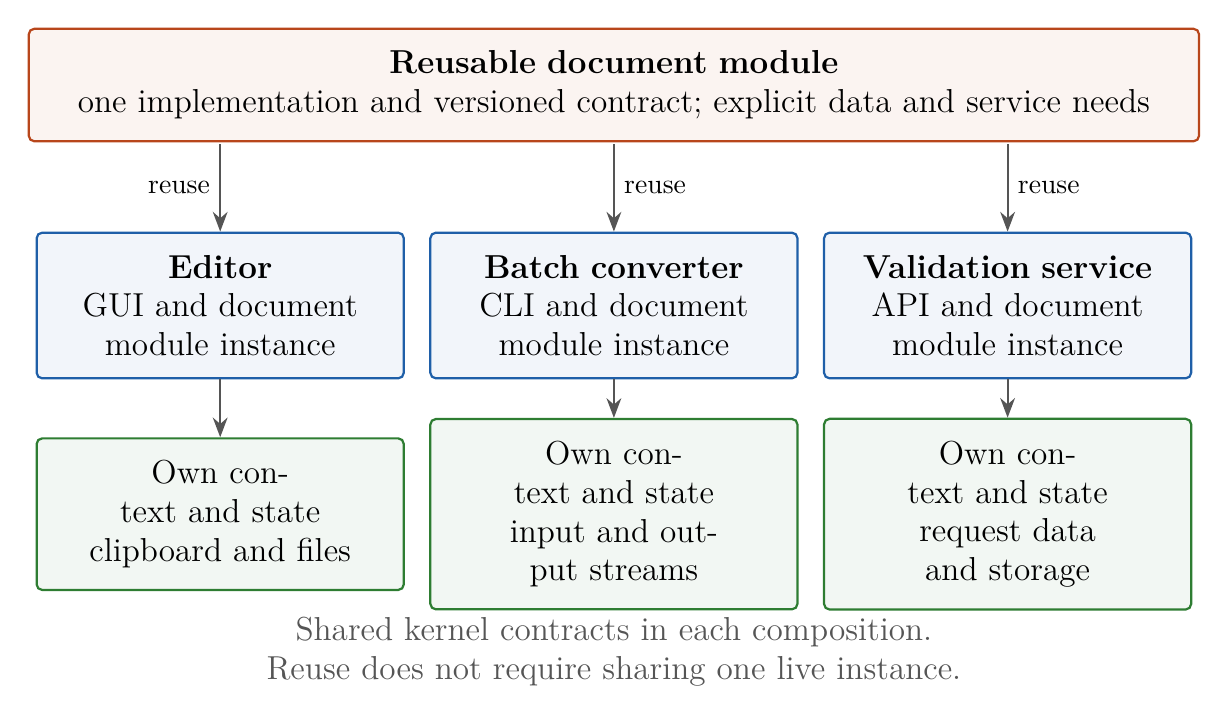
\begin{tikzpicture}[
  box/.style={draw,rounded corners=2pt,thick,align=center,inner sep=8pt,font=\large},
  host/.style={box,draw=elemA,fill=elemA!6,text width=4.1cm,minimum height=1.85cm},
  arrow/.style={-{Stealth[length=2.5mm]},thick,draw=frameline}
]
\node[box,draw=elemB,fill=elemB!6,text width=14.3cm,minimum height=1.2cm] (module) at (0,3.2)
  {\textbf{Reusable document module}\\one implementation and versioned contract; explicit data and service needs};
\node[host] (editor) at (-5,0.4) {\textbf{Editor}\\GUI and document\\module instance};
\node[host] (batch) at (0,0.4) {\textbf{Batch converter}\\CLI and document\\module instance};
\node[host] (service) at (5,0.4) {\textbf{Validation service}\\API and document\\module instance};
\draw[arrow] (-5,2.45) -- node[left,font=\normalsize] {reuse} (editor.north);
\draw[arrow] (0,2.45) -- node[right,font=\normalsize] {reuse} (batch.north);
\draw[arrow] (5,2.45) -- node[right,font=\normalsize] {reuse} (service.north);
\foreach \x/\name/\desc in {-5/editor/clipboard and files,0/batch/input and output streams,5/service/request data and storage} {
  \node[box,draw=elemC,fill=elemC!6,text width=4.1cm,minimum height=1.9cm] (state\name) at (\x,-2.25)
    {Own context and state\\\desc};
  \draw[arrow] (\name.south) -- (state\name.north);
}
\node[align=center,text=frameline,font=\large,text width=14.4cm] at (0,-4)
  {Shared kernel contracts in each composition.\\Reuse does not require sharing one live instance.};
\end{tikzpicture}
\end{document}
